% -*-latex-*-
%\documentclass[dvips,handout]{beamer}  %% handout
\documentclass[dvips,12pt]{beamer}    %% presentation
\usepackage{etex,pictex}
%\usepackage{pstricks,pst-plot}
%\setlength{\topmargin}{-1.7in}
\setbeamercovered{transparent}
\title{Diffusion Wave Hypothesis}
\author{Alan R. Rogers}
\date{\today}
\begin{document}
\frame{\titlepage}

\frame{\frametitle{Neandertal \& Modern}
\begin{center}
 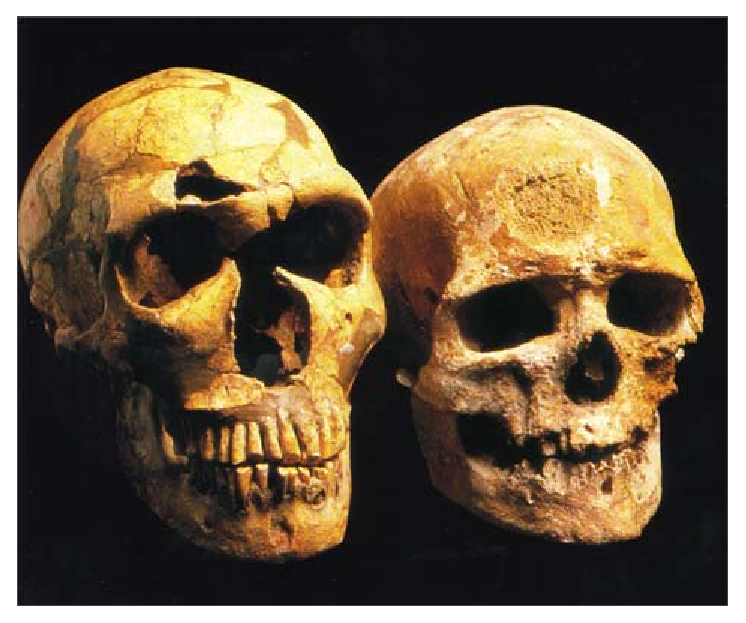
\includegraphics[height=0.7\textheight]{nean_mod.eps}
\end{center}
}

\begin{frame}
\frametitle{Moderns invade Eurasia}
\centering
 \includegraphics[width=\textwidth]{modhummap.eps}
\end{frame}

\frame{\frametitle{Moderns made fancy points}
\centering
 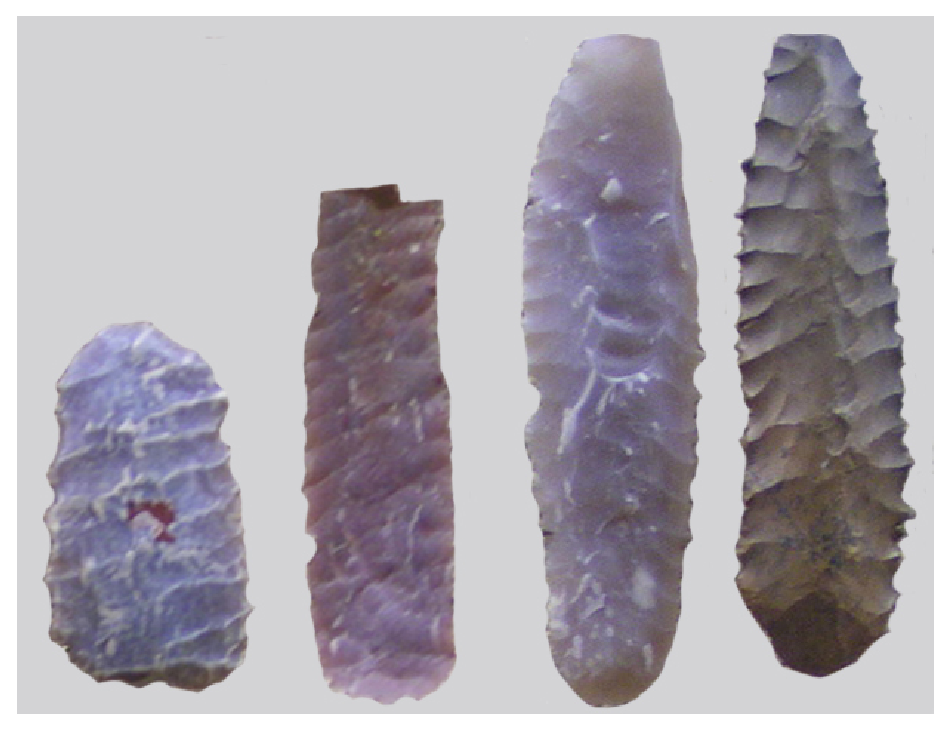
\includegraphics[width=\textwidth]{solutrean.eps}
}

\frame{\frametitle{Spear throwers}
\centering
 \includegraphics[height=0.7\textheight]{atlatl.ps}
}

\frame{\frametitle{Art}
\centering
 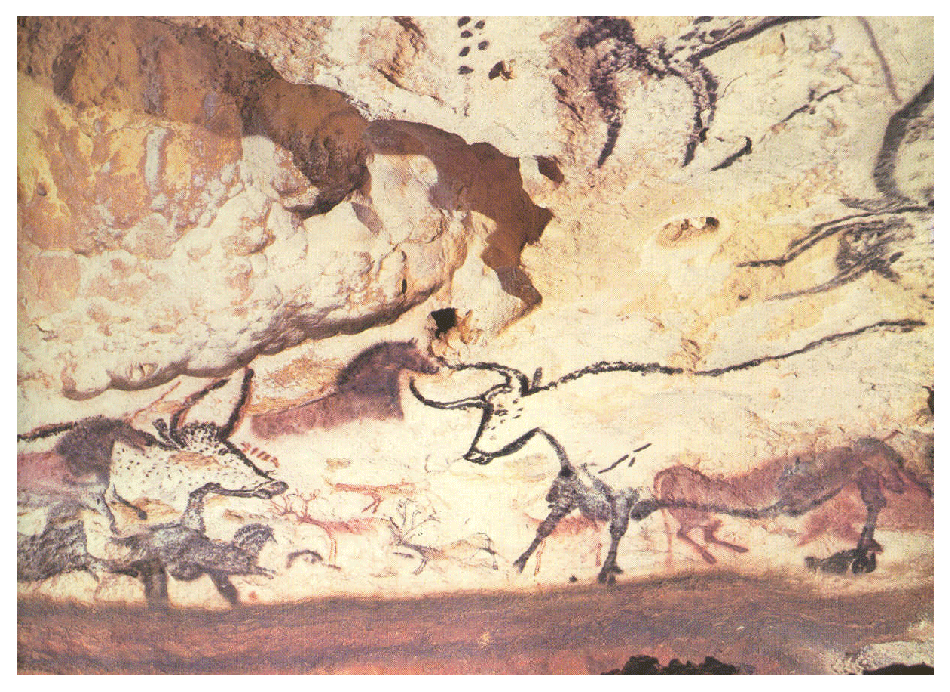
\includegraphics[height=0.7\textheight]{lascaux2.eps}
}

%\frame{\frametitle{Pace of change}
%\begin{itemize}
%\item slow before moderns arrive
%\item fast thereafter
%\end{itemize}
%}

\frame{\frametitle{How did modern humans evolve?}
In the 1980s and 90s, there were two main hypotheses
\begin{itemize}
\item Multiregional
\item Replacement
\end{itemize}
}

\begin{frame}
\frametitle{Multiregional hypothesis}
\begin{columns}
\column{0.5\textwidth}
\includegraphics[height=0.7\textheight]{multireg.ps}
\column{0.5\textwidth}
\begin{itemize}
\item<+-| alert@+> \emph{Homo erectus} expands into Eurasia 1.8~mya
\item<+-| alert@+> Strong gene flow
\item<+-| alert@+> Favorable mutations spread in every direction.
\item<+-| alert@+> Moderns have no geographic origin.
\end{itemize}
\end{columns}
\end{frame}

\begin{frame}
\frametitle{Replacement hypothesis}
\begin{columns}
\column{0.5\textwidth}
\includegraphics[height=0.7\textheight]{replacement.ps}
\column{0.5\textwidth}
\begin{itemize}
\item<+-| alert@+> \emph{Homo erectus} expands into Eurasia 1.8~mya
\item<+-| alert@+> Moderns evolve in Africa by 100~kya
\item<+-| alert@+> Expand into Eurasia btw 100 and 30~kya
\item<+-| alert@+> No mixing with archaics
\end{itemize}
\end{columns}
\end{frame}

\frame{\frametitle{Mitochondrial story, circa 1996}
This problem has been studied using bones, stones, and genes.
Here's how I would have summarized the genetic evidence:
\begin{itemize}
\item<+-| alert@+> Population expansion 50--100~kya
\item<+-| alert@+> Early population $\leq 5000$ females
\item<+-| alert@+> Late population $\geq \hbox{1,000,000}$ females
\item<+-| alert@+> Consistent with replacement hypothesis
\item<+-| alert@+> but not multiregional hypothesis
\end{itemize}
}

\begin{frame}
\frametitle{Nuclear genes}
Since 1997, we have relied more and more on nuclear genes.
\end{frame}

\begin{frame}
\frametitle{Some nuclear loci have shallow genealogies}
\begin{columns}
\column{0.65\textwidth}
\includegraphics[width=\textwidth]{underhilltree.eps}\\
\textsc{\small (Underhill \& al 2000)}
\column{0.35\textwidth}
\begin{block}{Y chromosome}
49~kyr old

\pause
Old branches are short;
\pause
suggests expansion.

\pause
Supports replacement hypothesis. 
\end{block}
\end{columns}
\end{frame}

\begin{frame}
\frametitle{Others have deep genealogies}
\begin{columns}
\column{0.65\textwidth}
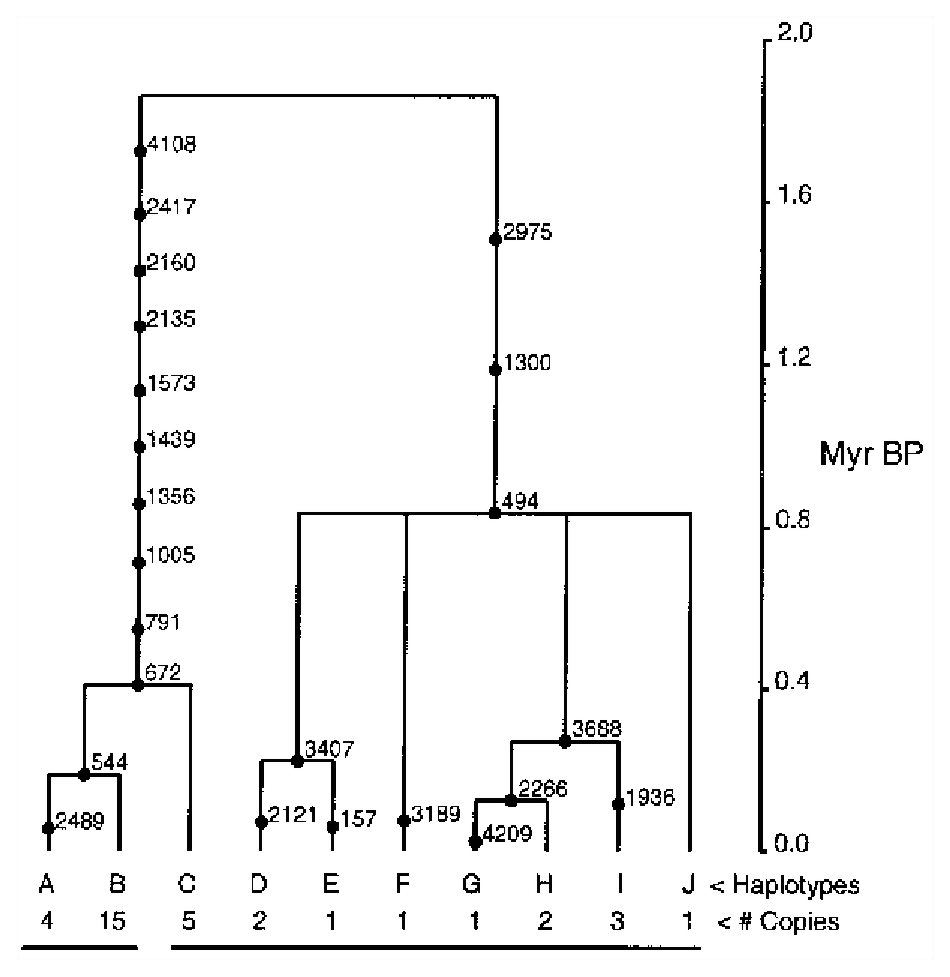
\includegraphics[width=\textwidth]{pdha1tree.eps}
\column{0.35\textwidth}
\begin{block}{PDHA1 locus {\small (Harris \& Hey 1999)}}
\pause
Nearly 2~myr old.

\pause 
Old branches long.

\pause
Suggests subdivision.

\pause
Supports multiregional hypothesis 
\end{block}
\end{columns}
\end{frame}

\begin{frame}
\frametitle{The puzzle}
Some nuclear loci support one hypothesis; 
\pause
some support the other.

\bigskip
\pause
The truth must somehow encompass both.
\end{frame}

\begin{frame}
\frametitle{Diffusion wave authors}
Vinayak Eswaran\hfill Henry Harpending\\
\begin{columns}
\column{0.5\textwidth}
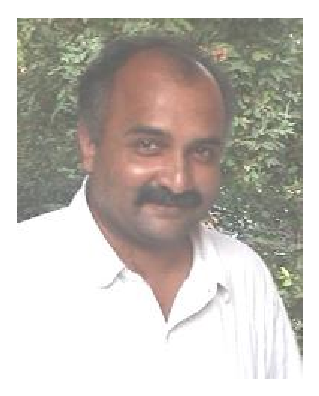
\includegraphics[width=\textwidth]{VEswaran.eps}%
\column{0.5\textwidth}
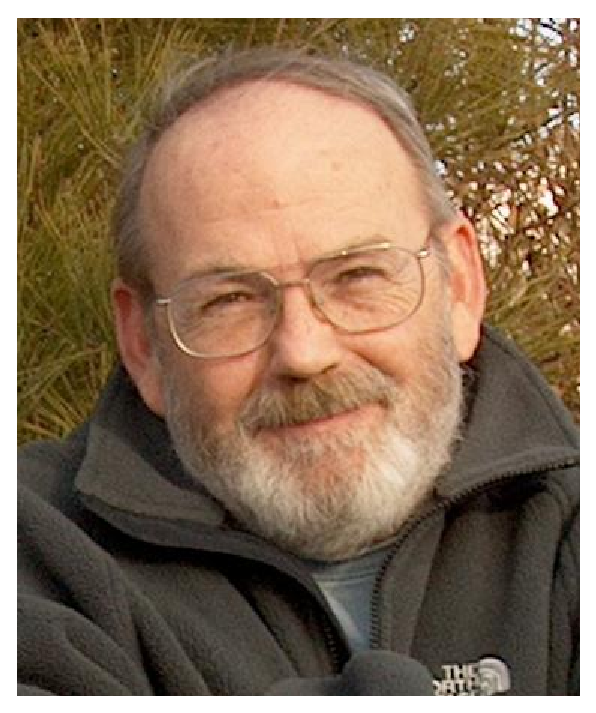
\includegraphics[width=\textwidth]{hch.eps}%
\end{columns}
\end{frame}

%\begin{frame}
%\frametitle{Maybe a trickle of admixture?}
%\centering
%\includegraphics[width=\textwidth]{models-hodgson08.eps}
%\end{frame}

\begin{frame}
\frametitle{Diffusion wave hypothesis}
\begin{itemize}
\item \emph{Homo erectus} expands into Eurasia 1.8~mya
\pause
\item Moderns evolve in Africa by 100~kya
\pause
\item Expand into Eurasia btw 100 and 30~kya
\pause
\item Some mixing with archaics
\pause
\item Co-adapted gene complex reduces fitness of hybrids.
\end{itemize}
\end{frame}

\begin{frame}
\frametitle{Co-adapted gene complexes}
\begin{itemize}
\item Hybrids often have low fitness
\pause
\item Especially when population is deeply subdivided
\pause
\item Probably because each sub-population has evolved a
     different ``co-adapted gene complex.''
\item Co-adapted gene complex: a group of alleles at
     different loci that work well together, but not apart.
\item For example, the parts in your Toyota work well
     together, but don't install them in your Ford.
\end{itemize}
\end{frame}

\begin{frame}
\frametitle{Copepod \emph{Tigriopus californicus}}
\begin{columns}
\column{0.5\textwidth}
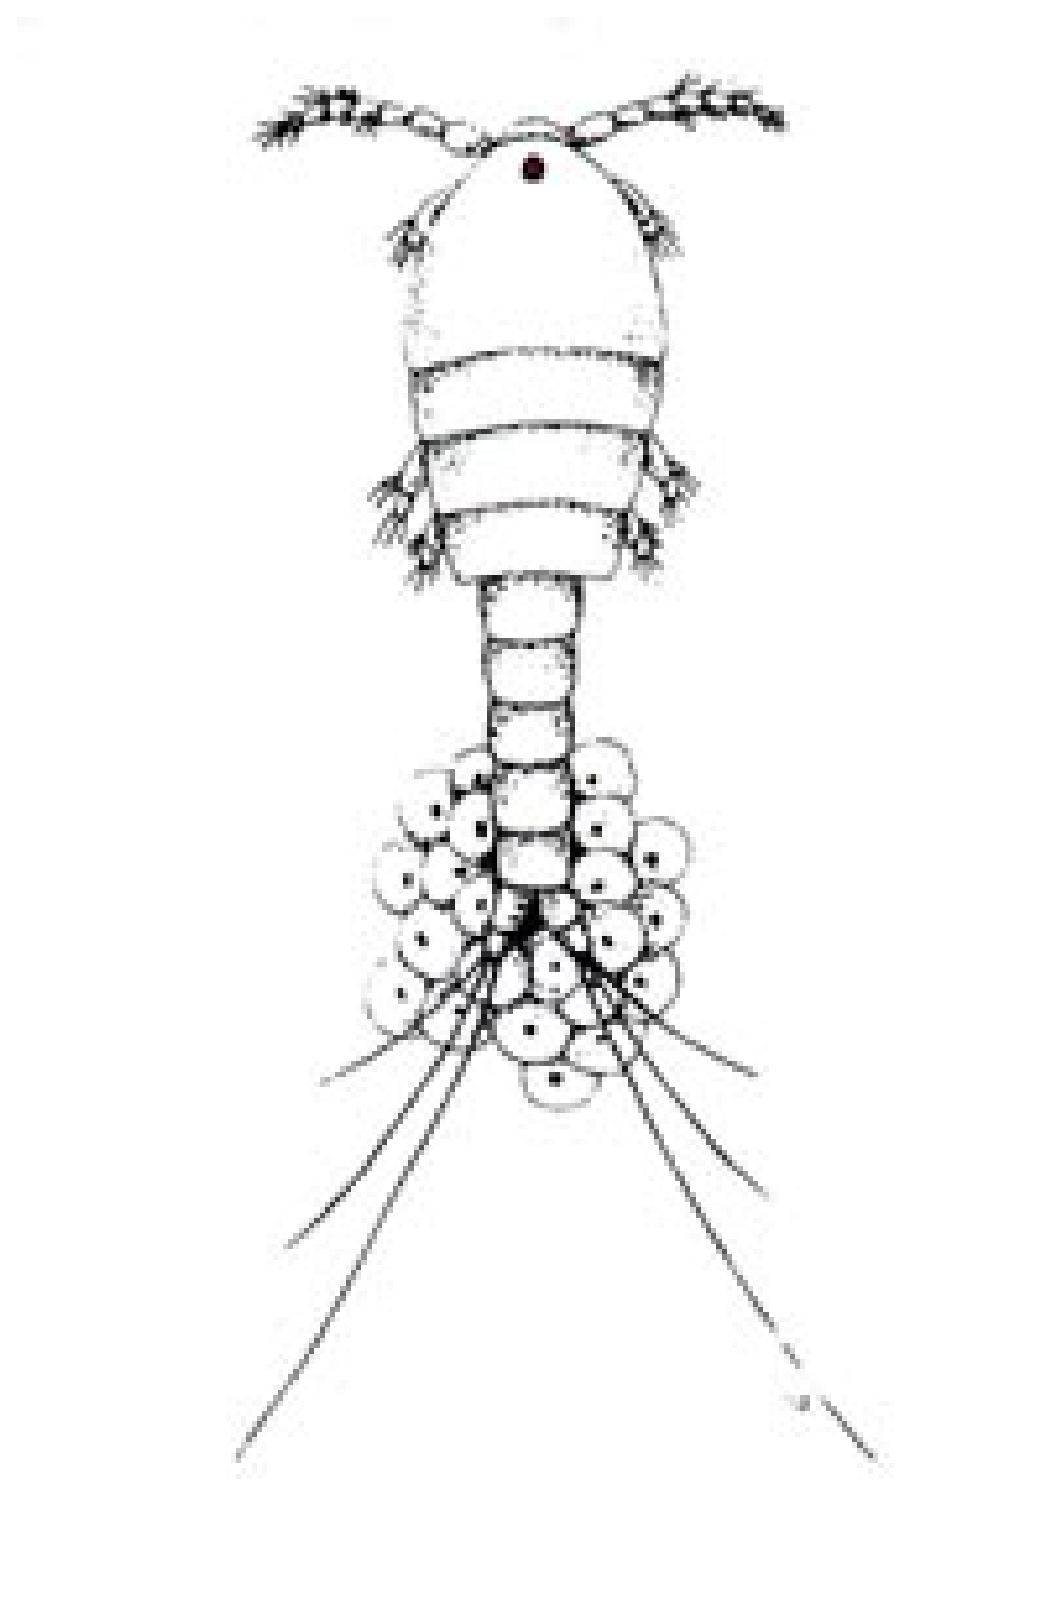
\includegraphics[width=\textwidth]{tigriopus.ps}
\column{0.5\textwidth}
\begin{itemize}
\pause
\item Live in tide pools
\pause
\item Isolated populations
\pause
\item Hybrids have low fitness
\pause
\item Different complexes of coadapted alleles
\end{itemize}
\end{columns}
\end{frame}


\begin{frame}
\frametitle{Modelling a co-adapted gene complex}
\begin{itemize}
\item Several unlinked loci
\pause
\item Each locus has a ``modern'' and an ``archaic'' allele.
\item Modern individuals have 2 copies of the modern
     allele at each locus.  All others are archaic.
\pause
\item Moderns have a selective advantage.
\pause
\item Advantage disappears if you have even 1 copy of an
     archaic allele
\end{itemize}
\end{frame}

\begin{frame}
\frametitle{Neutral loci}
\begin{itemize}
\item
There are 40 unlinked neutral loci, in addition to the co-adapted gene
complex. 
\pause
\item
The statistics we report are based on these neutral loci, not on the
co-adapted gene complex.
\end{itemize}
\end{frame}

\begin{frame}
\frametitle{Progress of diffusion wave}
\mbox{%
\small
\def\hunit{0.007\textwidth}
\def\vunit{0.1\textwidth}
\beginpicture
%\setcoordinatesystem units <.03in, 0.5in> point at 0 0
\setcoordinatesystem units <\hunit, \vunit> point at 0 0
\setplotarea x from 0 to 100, y from 0 to 1
\axis left 
   ticks numbered from 0.0 to 1.0 by 0.5 /
\axis bottom ticks numbered from 0 to 100 by 50 /
%Generation 1000: 
\put {\small Gen 1000} [tr] at 100 0.9
\plot
 1	1
29	1
30	0.89
31	0.77
32	0.34
33	0.03
34	0
98	0
/
\setcoordinatesystem units <\hunit, \vunit> point at 0 1.6
\setplotarea x from 0 to 100, y from 0 to 1
\axis left label {\lines{Modern\cr fraction}}
   ticks numbered from 0.0 to 1.0 by 0.5 /
\axis bottom ticks numbered from 0 to 100 by 50 /
%Generation 2000: 
\put {\small Gen 2000} [tr] at 100 0.9
\plot
 1	1
54	1
55	0.81
56	0.51
57	0.39
58	0.01
59	0
98	0
/
\setcoordinatesystem units <\hunit, \vunit> point at 0 3.2
\setplotarea x from 0 to 100, y from 0 to 1
\axis left 
   ticks numbered from 0.0 to 1.0 by 0.5 /
\axis bottom label {Location} ticks
  numbered from 0 to 100 by 50 /
%Generation 3000: 
\put {\small Gen 3000} [tr] at 100 0.9
\plot
 1	1
75	1
76	0.97
77	0.92
78	0.62
79	0.36
80	0.25
81	0.05
82	0.1
83	0.01
84	0
98	0
/
\endpicture}

\end{frame}

\begin{frame}
\frametitle{Fraction of neutral loci that are African, after diffusion wave}
\mbox{%
\def\hunit{0.007\textwidth}
\def\vunit{0.4\textwidth}
\small
\beginpicture
%\setcoordinatesystem units <\hunit, 2in>
\setcoordinatesystem units <\hunit, \vunit>
\setplotarea x from 0 to 100, y from 0 to 1
\axis left label {\lines{African\cr fraction}}
   ticks numbered from 0.0 to 1.0 by 0.5 /
\axis bottom 
  label {Location} ticks
  numbered from 0 to 100 by  25 /
%deme admixture C=4
\setbox0=\hbox{$\swarrow$}%
\put {$\swarrow$ \raise \ht0 \hbox{4 coadapted loci}} [bl] <3pt,3pt> at 25 0.4872
\plot
   0         1
   1    0.9728
   2    0.9565
   3    0.9349
   4    0.9032
   5    0.8922
   6    0.8635
   7    0.8348
   8    0.8089
   9    0.7928
  10    0.7649
  11    0.7423
  12    0.7175
  13    0.6954
  14    0.6677
  15    0.6609
  16    0.6437
  17    0.6207
  18    0.6017
  19    0.5793
  20    0.5643
  21    0.5464
  22    0.5347
  23    0.5135
  24    0.4975
  25    0.4872
  26     0.473
  27    0.4594
  28    0.4402
  29    0.4198
  30    0.4048
  31     0.388
  32    0.3727
  33    0.3619
  34    0.3348
  35    0.3283
  36    0.3288
  37    0.3222
  38    0.3099
  39    0.2958
  40    0.2933
  41    0.2807
  42    0.2733
  43    0.2619
  44    0.2477
  45    0.2358
  46    0.2155
  47    0.2167
  48     0.214
  49    0.2071
  50    0.2023
  51    0.1994
  52      0.19
  53    0.1878
  54     0.179
  55    0.1704
  56     0.169
  57    0.1611
  58    0.1609
  59    0.1496
  60     0.145
  61    0.1384
  62    0.1302
  63    0.1302
  64    0.1261
  65    0.1257
  66    0.1195
  67    0.1197
  68    0.1177
  69    0.1171
  70    0.1127
  71      0.11
  72    0.1031
  73   0.09788
  74   0.09572
  75   0.09007
  76   0.08769
  77   0.08436
  78   0.08236
  79   0.07781
  80   0.07244
  81   0.07117
  82   0.07237
  83   0.07121
  84   0.06734
  85   0.06581
  86   0.06805
  87   0.06531
  88   0.06443
  89   0.06189
  90   0.05968
  91   0.06098
  92   0.05962
  93   0.05855
  94   0.06071
  95   0.05539
  96   0.05506
  97   0.05818
/
% C=8
\put {$\swarrow$ \raise \ht0 \hbox{8 coadapted loci}} [bl] <3pt,3pt> at 50 0.8042
\setdashes
\plot
   0         1
   1    0.9963
   2    0.9937
   3    0.9926
   4    0.9901
   5    0.9877
   6    0.9836
   7    0.9812
   8    0.9773
   9    0.9754
  10    0.9707
  11    0.9681
  12    0.9659
  13    0.9616
  14    0.9578
  15    0.9551
  16    0.9534
  17    0.9511
  18    0.9456
  19    0.9425
  20    0.9401
  21    0.9344
  22    0.9307
  23    0.9271
  24    0.9256
  25    0.9236
  26    0.9188
  27    0.9151
  28    0.9032
  29    0.8974
  30    0.8938
  31    0.8876
  32    0.8822
  33    0.8786
  34    0.8701
  35    0.8613
  36     0.861
  37    0.8597
  38    0.8494
  39    0.8458
  40    0.8319
  41    0.8248
  42    0.8262
  43    0.8176
  44    0.8193
  45     0.817
  46    0.8108
  47    0.8052
  48    0.8086
  49    0.8084
  50    0.8042
  51     0.798
  52    0.7974
  53    0.7962
  54    0.7931
  55    0.7881
  56    0.7829
  57     0.781
  58    0.7807
  59    0.7818
  60      0.78
  61    0.7789
  62     0.777
  63    0.7696
  64    0.7712
  65    0.7671
  66    0.7678
  67    0.7634
  68    0.7622
  69    0.7636
  70    0.7639
  71    0.7634
  72    0.7614
  73    0.7606
  74    0.7609
  75    0.7573
  76    0.7529
  77    0.7484
  78    0.7431
  79    0.7406
  80    0.7412
  81    0.7377
  82    0.7315
  83    0.7313
  84    0.7294
  85    0.7302
  86     0.721
  87    0.7173
  88    0.7134
  89    0.7118
  90    0.7118
  91     0.708
  92    0.7036
  93    0.6998
  94    0.7002
  95    0.6999
  96    0.6977
  97    0.6919
/
\endpicture}

\end{frame}

\begin{frame}
\frametitle{Diffusion wave predicts archaic admixture at some
(but not all) loci.} 

\begin{itemize}
\pause
\item At few loci if adaptation is complex.
\pause
\item At many loci if adaptation is simple.
\end{itemize}
\pause
Just the sort of confusion that we see in real data.

\pause
\medskip
Next$\ldots$ the evidence
\end{frame}

\begin{frame}
\frametitle{Tajima's D}
\begin{itemize}
\item  a statistic that is sensitive
  both to selection and population growth.

\pause
\item behaves differently under the replacement,
  multiregional, and diffusion wave hypotheses.
\end{itemize}
\end{frame}

\begin{frame}
\frametitle{Replacement hypothesis}
 \begin{columns}
\column{0.7\textwidth}
 \includegraphics[width=\textwidth]{piDrepl.ps}
\column{0.3\textwidth}
\raggedright
Simulated Tajima's D 
\begin{itemize}
\pause
\item Many near --2.\\
\pause
\item None much above --1.
\end{itemize}
\end{columns}
\end{frame}

\begin{frame}
\frametitle{Multiregional hypothesis}
\begin{columns}
\column{0.7\textwidth}
 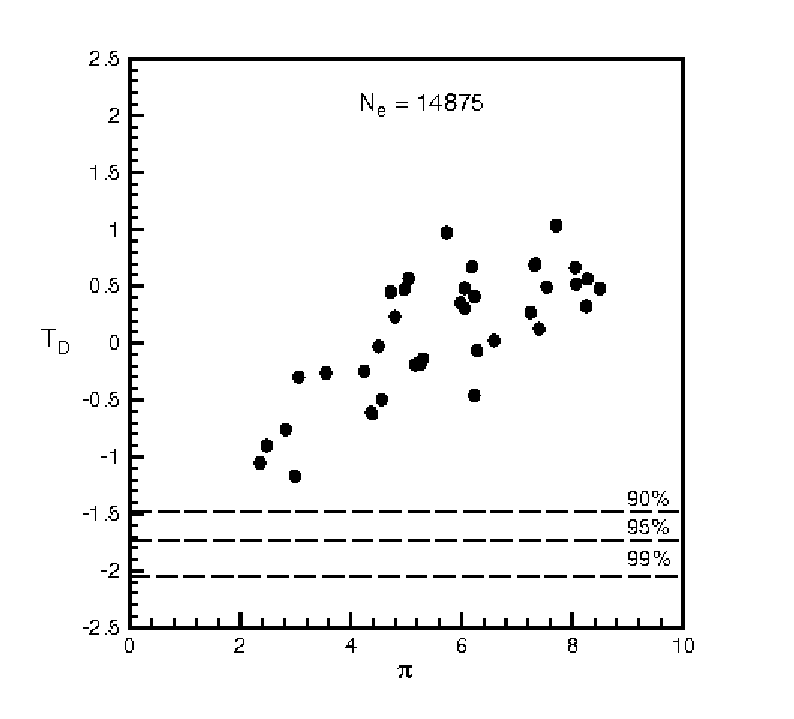
\includegraphics[width=\textwidth]{piDmre.eps}
\column{0.3\textwidth}
\raggedright
Simulated Tajima's D 
\begin{itemize}
\pause
\item Symmetric about zero\\
\pause
\item Would be $>0$ with less migration
\end{itemize}
\end{columns}
\end{frame}

\begin{frame}
\frametitle{Multiregional hypothesis again}
\begin{columns}
\column{0.7\textwidth}
 \includegraphics[width=\textwidth]{piDmre2.ps}
\column{0.3\textwidth}
\raggedright
Simulated Tajima's D 
\begin{itemize}
\item With more population structure\\
\pause
\item Average above zero.\\
\end{itemize}
\end{columns}
\end{frame}

\begin{frame}
\frametitle{Diffusion Wave Hypothesis}
\begin{columns}
\column{0.7\textwidth}
\includegraphics[width=\textwidth]{piDdiffwave.ps}
\column{0.3\textwidth}
\raggedright
Simulated Tajima's D 
\begin{itemize}
\pause
\item   From --2 to +1.5.
\pause
\item   Most are negative.
\end{itemize}
\end{columns}
\end{frame}

\begin{frame}
\frametitle{Reality}
\begin{columns}
\column{0.7\textwidth}
 \includegraphics[width=\textwidth]{piDStephens.ps}
\column{0.3\textwidth}
\raggedright
Observed Tajima's D {\small(Stephens et al 2003)}
\begin{itemize}
\pause
\item Too negative for multiregional hypothesis.\\
\pause
\item Not negative enough for replacement hypothesis.
\end{itemize}
\end{columns}
\end{frame}

\frame{\frametitle{Summary of Tajima's D}
Explains the pattern in the data better than any other
hypothesis.

\bigskip

\onslide<2>
If this hypothesis is correct, many human loci should have archaic
admixture.  How can we tell?
}

\begin{frame}
\frametitle{More disequilibrium in Europe than Africa}
\begin{columns}
\column{0.6\textwidth}
 \includegraphics[width=\textwidth]{ldcurve.ps}
\column{0.4\textwidth}
\raggedright
\begin{itemize}
\onslide<+->
\item More LD in Europe than Africa
\onslide<+->
\item Could reflect archaic admixture in Europe
\onslide<+->
\item or a European bottleneck.
\end{itemize}
\textsc{\footnotesize (Reich et al 2001)}
\end{columns}
\end{frame}

\begin{frame}
\frametitle{Decay of LD with distance along chromosome}
\includegraphics[width=\textwidth]{Jacobsson-LDdecay.eps}
\end{frame}

\begin{frame}
\frametitle{LD increases with distance from Africa}
\includegraphics[height=0.6\textheight,width=\textwidth]{Jacobsson-LDdist.eps}
\end{frame}

\frame{\frametitle{Disequilibrium at locus RRM2P4}
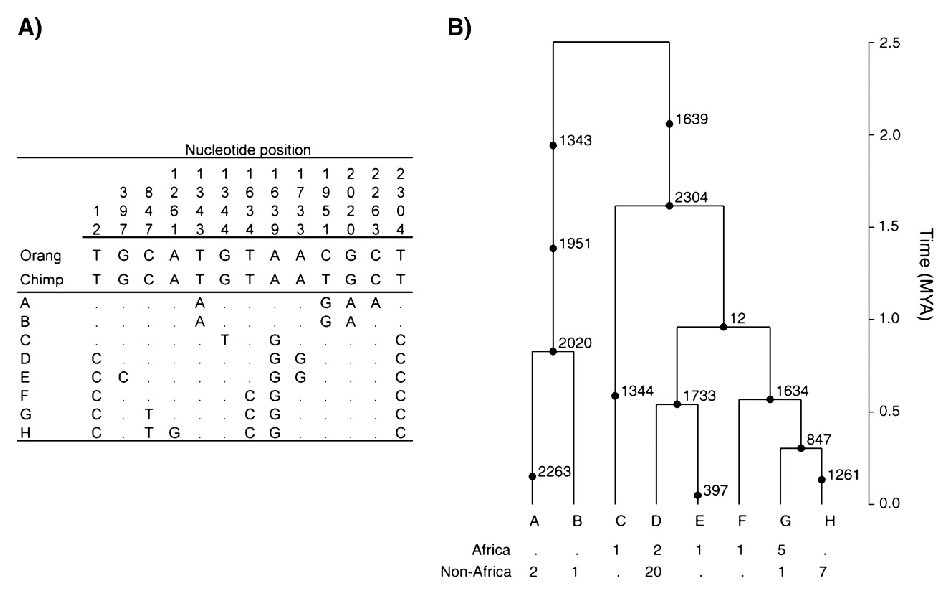
\includegraphics[width=\textwidth]{rrm2p4.eps}\\
\textsc{\footnotesize (Garrigan et al 2004)}
}

\begin{frame}
\frametitle{RRM2P4 continued}
\begin{columns}
\column{0.6\textwidth}
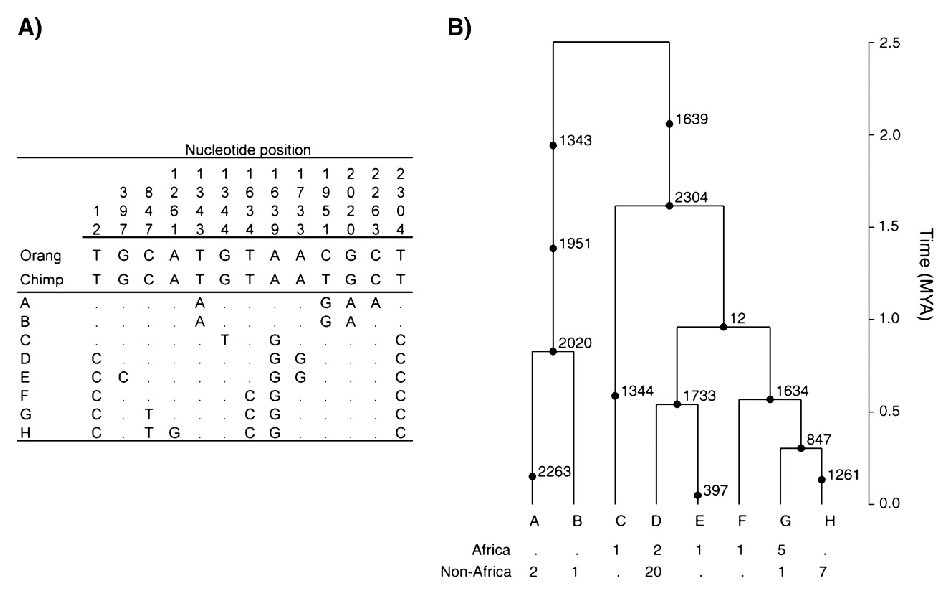
\includegraphics[width=\textwidth]{rrm2p4.eps}\\
\textsc{\footnotesize (Garrigan et al 2004)}
\column{0.4\textwidth}
\raggedright
\begin{itemize}
\item<alert@1> H'types A,B in strong disequilibrium
\item<alert@1> No surprise: sequence is short (2.4~kb)
\item<alert@2> Locus is very old: 2.5~myr
\end{itemize}
\end{columns}
\end{frame}

\begin{frame}
\frametitle{Deep disequilibrium at locus Xp21.1}
\begin{columns}
\column{0.6\textwidth}
\footnotesize
\renewcommand{\arraystretch}{0.7}
\begin{tabular}{cc@{}c@{}c@{}c@{}c@{}c@{}cc@{}c@{}c@{}c@{}c@{}c@{}cc@{}c@{}c@{}c@{}c@{}c@{}c@{}c@{}c@{}c}
          &  & & & & & & &  & & & & & & & 1&1&1&1&1&1&1&1&1&1\\
          &  & & & &1&1&1& 8&8&9&9&9&9&9& 5&5&5&5&6&6&6&6&7&7\\
          & 1&2&4&7&0&2&3& 4&5&2&3&4&4&6& 4&4&5&6&0&4&6&6&3&3\\
          & 5&1&3&3&6&9&1& 9&0&7&1&0&9&3& 5&6&4&6&8&2&3&4&4&6\\
          & 5&7&0&8&9&0&6& 1&2&4&6&4&5&8& 2&3&8&0&0&6&5&1&8&5\\
\hline
    a     & .&.&.&t&.&.&a& c&.&a&.&.&.&.& .&a&a&.&.&.&.&a&.&.\\
    b     & .&c&.&t&.&.&.& .&.&a&.&.&.&.& c&a&a&.&.&.&.&a&.&.\\
    C     & .&.&G&.&T&C&.& .&G&.&.&.&.&G& .&.&.&.&T&.&.&.&T&C\\
    d     & .&.&.&t&.&.&.& .&.&a&.&.&.&.& .&a&a&.&.&.&.&a&.&.\\
    e     & .&.&.&t&.&.&.& c&.&a&.&.&.&.& .&a&a&.&.&.&.&a&t&c\\
    f     & .&.&.&t&.&.&.& .&.&a&.&.&.&.& .&a&a&.&.&.&.&a&t&c\\
    g     & c&.&.&t&.&.&.& .&.&a&.&.&.&g& .&a&a&.&.&.&g&a&t&c\\
    h     & c&.&.&t&.&.&.& .&.&a&.&t&g&.& .&a&a&.&.&.&g&a&t&c\\
    i     & c&.&.&t&.&.&.& .&.&a&.&.&g&.& .&a&a&.&.&.&g&a&t&c\\
    j     & c&.&.&t&.&.&.& .&.&a&.&.&.&.& .&a&a&.&.&.&g&a&t&c\\
    k     & c&.&.&t&.&.&.& .&.&a&.&.&g&.& .&a&a&.&.&.&.&a&t&c\\
    l     & c&.&.&t&.&.&.& .&.&a&.&.&g&.& .&a&a&g&.&.&g&a&t&c\\
    m     & .&.&.&t&.&.&a& c&.&a&.&.&.&.& .&a&a&.&.&c&.&a&.&.\\
    n     & .&.&.&t&.&.&.& c&.&a&g&.&.&.& .&a&a&.&.&.&.&a&.&.\\
    o     & .&.&.&t&.&.&.& .&.&a&g&.&.&.& .&a&a&.&.&.&.&a&.&.\\
    p     & .&.&.&t&.&.&.& c&.&a&.&.&.&.& .&a&a&.&.&.&.&a&.&c\\
    q     & c&.&.&t&.&.&.& .&.&a&g&.&g&.& .&a&a&.&.&.&g&a&t&c\\
\end{tabular}%
\column{0.4\textwidth}
\raggedright
\begin{itemize}
\item Sequence is 17.5~kb long
\pause
\item MRCA is 1.9~myr old
\pause
\item H'type C in strong disequilibrium
\pause
\item Not balancing selection: too much disequilibrium
\pause
\item Requires isolated populations

\textsc{(Garrigan et al 2005)}
\end{itemize}
\end{columns}
\end{frame}

\frame{\frametitle{Microcephalin (Evans et al 2006)}
\begin{itemize}
\item Sequenced a large (23.4~kb) region.
\pause
\item One haplotype has been increasing for 37~kyr.
\pause
\item In ``near-complete LD across the entire region.''
\pause
\item MRCA 1.7~mya
\pause
\item Can't be balancing selection (too much LD).
\pause
\item Suggests archaic admixture.
\end{itemize}
}

\frame{\frametitle{Current views}
\begin{itemize}
\item Everyone agrees that there was little or no admixture of neutral
  archaic alleles.
\item Neanderthal alleles are different at several nuclear
  protein-coding loci.
\item Authors disagree about the likelihood of adaptive introgression.
\item We still don't know.
\end{itemize}
}

\frame{\frametitle{Update: 2010} Neandertal genome (Green et al 2010)
  indicates that non-African populations have some Neandertal
  ancestry.

\centering
\begin{tabular}{lcc}
           & Neandertal\\
Population & ancestry (\%)&S.E.\\ \hline
French     & 1.7 & 0.3\\
Han Chinese & 2.0 & 0.3\\
Papuan     & 1.5 &0.3
\end{tabular}\\

\pause
\begin{itemize}
\item Equal Neandertal admixture outside Africa
\item None within Africa
\end{itemize}
}

\frame{\frametitle{Summary}
\begin{itemize}
\item Hypothesis: our ancestors expanded out of Africa 50~kya,
and mated with surrounding archaic populations.
\pause
\item Yet only a few archaic genes entered the modern population.
\pause
\item Explains the contradictory signals given by different
  genetic loci.
\pause
\item It also predicts that some nuclear genes should show signs of
  archaic admixture: deep gene trees and high LD.
\pause
\item We find this pattern at two loci: Xp21.1 and Microcephalin.
\pause
\item Are we part Neandertal?  The jury is still out.
\end{itemize}
}

\end{document}

